\documentclass{article}
\usepackage{amsmath}
\usepackage{amsfonts}
\usepackage{mathtools}
\usepackage{hyperref}
\usepackage[ruled]{algorithm2e}
\usepackage{graphicx}
\graphicspath{ {./images/} }
\usepackage{geometry}
\usepackage{float}
\usepackage[italian]{babel}
\geometry{a4paper, top=3cm, bottom=3cm, left=3cm, right=3cm}

\title{\textbf{Smoking study} \\
    \large Studio e analisi dei dati di soggetti fumatori e non}\\\\
\author{Natasha Fabrizio - Matricola: 717446 \\
Email: \textit{n.fabrizio@studenti.uniba.it} \\
    Francesco Saverio Cassano - Matricola: 716133 \\
Email: \textit{f.cassano45@studenti.uniba.it} \\\\
Documentazione realizzata in: \textbf{LaTeX} \\
Link repository GitHub: \textit{https://github.com/nat-asha117/progettoICON}\\\\
    Progetto di Ingegneria della Conoscenza}
    
\date{2021-2022}

\begin{document}

    \maketitle

    \newpage

    \tableofcontents{}

    \newpage

\section{Introduzione}

Il sistema è in grado di prevedere se un soggetto è potenzialmente un fumatore o meno, a seconda dei valori riscontrati nel dataset preso in considerazione. 
%

\noindent
Inoltre, l'utilizzatore del programma potrà inserire dei valori, (non necessariamente tutti) inerenti alle analisi, per poter comprendere se risulta un soggetto potenzialmente fumatore o meno; in caso affermativo, potrà ulteriormente decidere se ricevere o meno, un suggerimento su quali valori migliorare per non risultare più un fumatore.

\section{Requisiti funzionali}

La realizzazione del progetto è stata effettuata interamente in Python in quanto, tale linguaggio, risulta il più idoneo per la trattazione e analisi di dati; inoltre, è stato utilizzando come ambiente di lavoro l'IDE PyCharm 2022.

\subsection{Liberie utilizzate}
Le librerie Python utilizzate nel progetto, sono le seguenti:
\begin{itemize}
    \item \textbf{Matplotlib}: usata per la visualizzazione di tutti i grafici, presenti nel progetto.
    \item \textbf{Numpy}: usata per la visualizzazione di tutti i grafici, presenti nel progetto.
    \item \textbf{Pandas}: usata per l’importazione del  Dataset in formato ".csv".
    \item \textbf{Pgmpy}: usata per la creazione della rete bayesiana..
    \item\textbf{Scikit-learn}: usata per applicare i concetti del Machine Learning.
    \item \textbf{Warnings}: usata per la gestione dei messaggi  di warnings del sistema.
\end{itemize} 

\subsection{Installazione e avvio}

Per poter installare, correttamente, le librerie utilizzate:
\begin{itemize}
    \item aprire il terminale e navigare fino alla cartella dove è presente il file \textit{"main.py"}
    \item inserire il seguente comando : \textit{"pip install -r requirements.txt"}.
\end{itemize}
%
Per l'avvio del programma, sarà possibile trascinare il file \textit{"smoking.csv"} sopra il file \textit{"main.py"} oppure attraverso l'utilizzo del terminale, quest'ultimo aperto sul percorso dove è presente il file \textit{"main.py"} e successivamente, eseguire il comando \textit{"python main.py smoking.csv"}.
%

\noindent
Eventualmente, è possibile modificare il percorso di lettura del file .csv dal file \textit{"main.py"}, come segue da immagine:

\begin{figure}[H]
        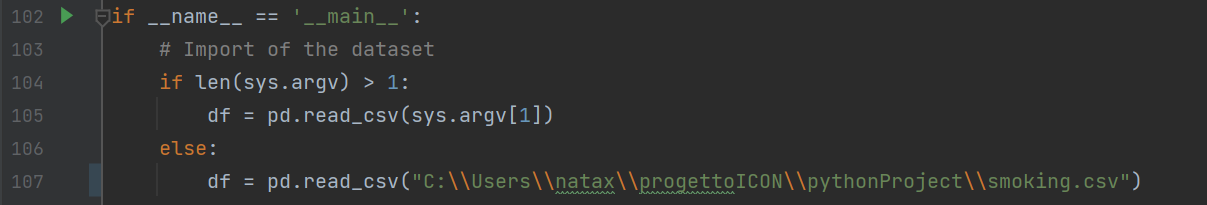
\includegraphics [width=0.8 cm + \textwidth]{modify}
        \centering
        \caption{Modifica del percorso di lettura del file csv a riga 107}
        \centering
\end{figure}

\section{Dataset}

Il dataset utilizzato, \textit{"Body signal of smoking"}, consiste in una raccolta di dati di segnali biologici sanitari di base. 
%
L'obiettivo è quello di determinare la presenza o l'assenza del fumo attraverso segnali biologici.
%
Link sorgente: \href{https://www.kaggle.com/datasets/kukuroo3/body-signal-of-smoking}{clicca qui}

\begin{figure}[H]
        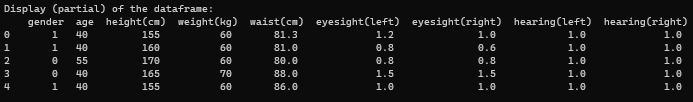
\includegraphics[width=0.9\textwidth]{display 1}
        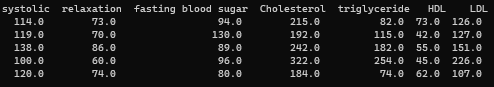
\includegraphics[width=0.9\textwidth]{display 2}
        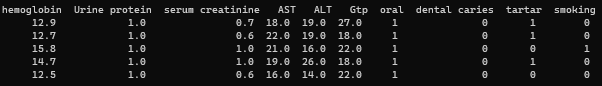
\includegraphics[width=0.9\textwidth]{display 3}
        \centering
        \caption{Anteprima del dataset}
        \centering
\end{figure}

\subsection{Preprocessing del dataset}
Nella fase di preprocessing, il dataset viene modificato in modo da poterlo utilizzare correttamente.\\
Il dataset non presenta problemi di mancanza dei dati.
\subsubsection{Feature dicotomiche}
Una feature dicotomica è una feature che presenta soltanto due modalità. 
Sono dicotomiche feature con valori come \{si, no\}, oppure \{vero, falso\}. In questo caso verranno assegnati i valori \{0,1\} rispettivamente alle due modalità, verrà sostituito
il valore iniziale della modalità con il nuovo valore assegnato. Nel nostro caso, le features dicotomiche sono:
\begin{itemize}
    \item \textbf{tartar}: \{vero, falso\} in \{0,1\}
    \item \textbf{oral}: \{vero, falso\} in \{0,1\}
    \item \textbf{gender}: \{vero, falso\} in \{0,1\}
\end{itemize}

\subsubsection{Features presenti nel dataset}
Per ridurre la complessità, si è scelto di eliminare la feature \textit{ID}, presente nel dataset, in quanto ha significatività bassa o tendendete a 0, essendo un semplice indice del dataset. 
Qui sotto sono elencante le features principali del dataset dopo la features selection:
\begin{itemize}
    \item \textbf{gender}
    \item \textbf{age} : 5 anni di intervallo
    \item \textbf{height(cm)} : 5 anni di intervallo
    \item \textbf{weight(kg)} : 5 anni di intervallo
    \item \textbf{waist(cm)} : lunghezza circonferenza vita
    \item \textbf{eyesight(left)}
    \item \textbf{eyesight(right)}
    \item \textbf{hearing(left)} 
    \item \textbf{hearing(right)}
    \item \textbf{systolic} : pressione sanguigna
    \item \textbf{relaxation} : pressione sanguigna
    \item \textbf{fasting blood sugar}
    \item \textbf{cholesterol} :  totale
    \item \textbf{triglyceride}
    \item \textbf{HDL} : tipo di colesterolo
    \item \textbf{LDL} : tipo di colesterolo
    \item \textbf{hemoglobin}
    \item \textbf{urine protein}
    \item \textbf{serum creatinine}
    \item \textbf{AST} : tipo glutammico ossalacetico transaminasi
    \item \textbf{ALT} : tipo glutammico ossalacetico transaminasi
    \item \textbf{Gtp} 
    \item \textbf{oral} : stato dell'esame orale
    \item \textbf{dental caries}
    \item \textbf{tartar} : stato tartaro
    \item \textbf{smoking}
\end{itemize}   

\subsection{Panoramica dei dati}
Mediante la stampa di una tabella, viene mostrato a schermo una panoramica inerente alle info del dataset.\\
\begin{figure}[H]
        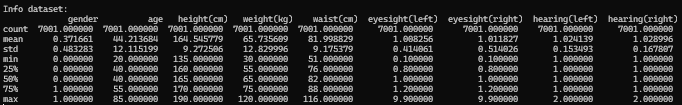
\includegraphics[width=0.9\textwidth]{info1}
        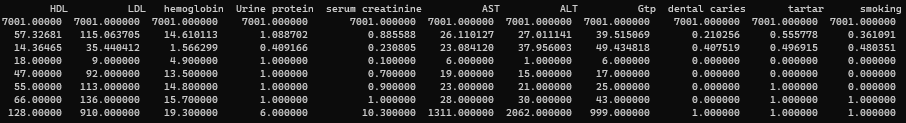
\includegraphics[width=0.9\textwidth]{info2}
        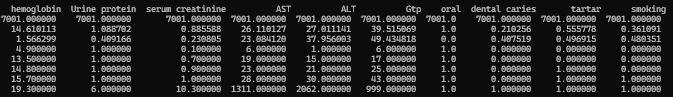
\includegraphics[width=0.9\textwidth]{info3}
        \centering
        \caption{Informazioni inerenti al dataset}
        \centering
\end{figure}

\subsection{Bilanciamento delle classi}
Attraverso un grafico, verifichiamo se il dataset sia ben bilanciato, in modo da riuscire ad avere ottimi risultati durante l'apprendimento.

\begin{figure}[H]
        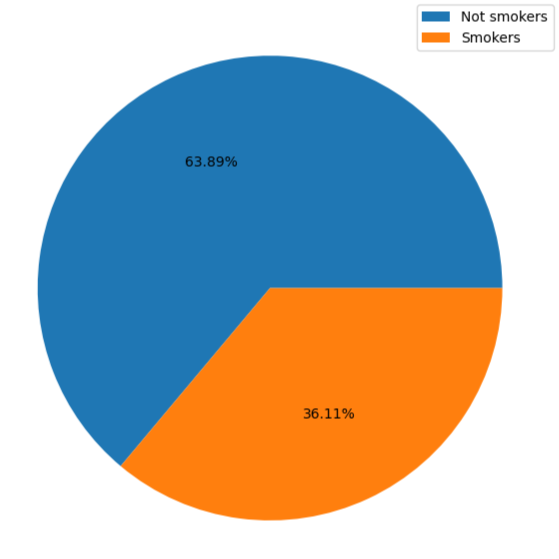
\includegraphics[width=7.5cm]{grafico1}
        \centering
        \caption{Grafico di occorrenze di fumatori e non fumatori}
        \centering
\end{figure}



\noindent
Dal grafico è possibile notare uno sbilanciamento delle classi.\\
Classi squilibrate mettono fuori gioco la \textit{"precisione"}. Questo è un problema sorprendentemente comune nell'apprendimento automatico (in particolare nella classificazione), che si verifica in set di dati con un rapporto sproporzionato di osservazioni in ciascuna classe.

\noindent
La precisione standard non misura più in modo affidabile le prestazioni, il che rende l'addestramento del modello molto più complicato. \par
\frenchspacing
\noindent
Vi sono diversi modi per poter risolvere il problema dello sbilanciamento delle classi. 
La soluzione per cui abbiamo optato è quella di utilizzare l'\textit{oversampling}. 
Per far ciò abbiamo individuato la classe di maggioranza e di minoranza ed abbiamo effettuato un resampling facendo combaciare le occorrenze.
Ottenendo, così, classi bilanciate:

\begin{figure}[H]
        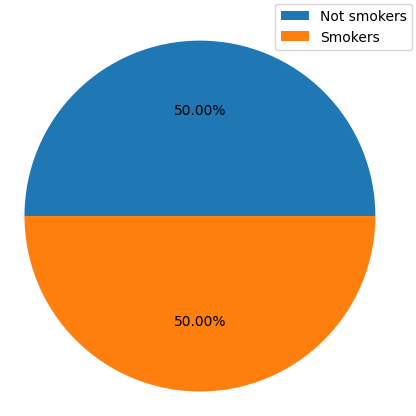
\includegraphics[width=7.6cm]{grafico2}
        \centering
        \caption{Grafico di occorrenze di fumatori e non fumatori dopo oversamplig}
        \centering
\end{figure}



\begin{figure}[H]
        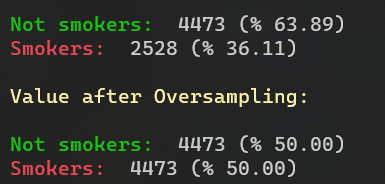
\includegraphics[width=0.9\textwidth]{value}
        \centering
        \caption{Bilanciamento classi}
        \centering
\end{figure}

\section{Apprendimento Supervisionato}
\subsection{Scelta del modello}
Per questo tipo di apprendimento abbiamo usato vari modelli per poi identificare quale fosse quello più adatto al nostro dataset. 
\\\\
I modelli valutati sono:
\begin{itemize}
    \item \textbf{KNN (K-Nearest Neighbors)}
    \begin{itemize} \item Il K-Nearest Neighbors, è un algoritmo utilizzato nel riconoscimento di pattern per la classificazione di oggetti basandosi sulle caratteristiche degli oggetti vicini a quello considerato.
    \end{itemize}
    \item \textbf{Decision Tree}
    \begin{itemize} \item Il Decision Tree è un classificatore con struttura ad albero (alberi di decisione), in cui ogni nodo può essere o foglia o nodo interno: se foglia, indica il valore della classe assegnata all’istanza; se nodo interno, specifica il test effettuato su un attributo. Per ciascun valore assunto da un attributo in un test, l’algoritmo crea un ramo e il relativo sottoalbero.
    \end{itemize}
    \item \textbf{Random Forest} 
    \begin{itemize} \item Il Random Forest è un classificatore d'insieme ottenuto dall'aggregazione tramite bagging di alberi di decisione. Esso si pone come soluzione che minimizza l'overfitting del training set rispetto agli alberi di decisione.
    \end{itemize}
    \item \textbf{SVC (Support-Vector Classification)}
    \begin{itemize} \item SVC è un modello di apprendimento per la regressione e la classificazione. Dato un insieme di esempi per l'addestramento, ognuno dei quali etichettato con la classe di appartenenza fra le due possibili classi, un algoritmo di addestramento per le SVC costruisce un modello che assegna i nuovi esempi a una delle due classi, ottenendo quindi un classificatore lineare binario non probabilistico.
    \end{itemize}
    \end{itemize}

\textbf{Classificatori Naïve Bayes}
\begin{itemize}
    \item \textbf{BernoulliNB (Bernoulli Naïve Bayes)}
    \begin{itemize} \item Questo classificatore è simile al multinomiale naive bayes ma i predittori sono variabili booleane. I parametri che usiamo per prevedere la variabile di classe occupano solo i valori sì o no.
    \end{itemize}
    \item \textbf{GaussianNB (Gaussian Naive Bayes)}
    \begin{itemize} \item Gaussian Naive Bayes è una variante di Naive Bayes che segue la distribuzione normale gaussiana e supporta dati continui.
    \end{itemize}
\end{itemize}
%
Sui suddetti abbiamo eseguito  il \textbf{K-Fold Cross Validation}, per verificare quale di esse fosse il più attendibile. In particolare, il \textbf{RepeatedKFold} con 5 ripetizioni, ottenendo così una media più accurata per le metriche.\\
Inoltre, le metriche di performance utilizzate nella valutazione sono:
\begin{itemize}
    \item accuratezza 
    \item precisione
    \item richiamo
    \item F1-score
\end{itemize}

Segue che i risultati medi ottenuti dalla valutazione sono:
\begin{figure}[H]
        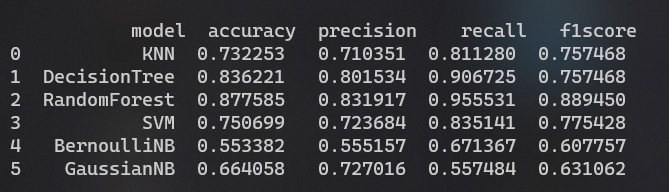
\includegraphics[width=0.9\textwidth]{imagModel}
        \centering
        \caption{Performance classificatori}
        \centering
\end{figure}

In particolare:

\begin{figure}[H]
        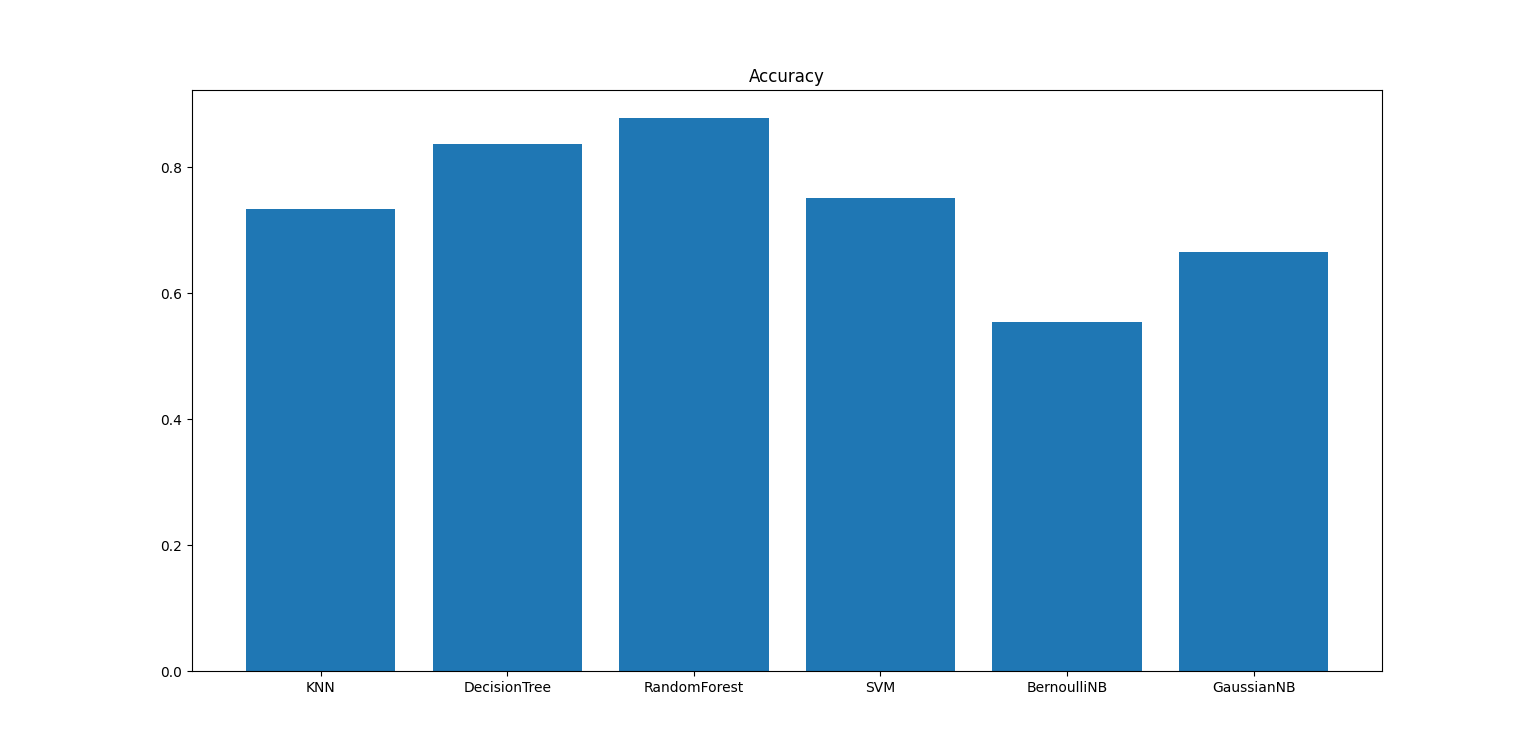
\includegraphics[width=0.9\textwidth]{Accuracy}
        \centering
        \caption{Grafico metrica accuratezza}
        \centering
\end{figure}

\begin{figure}[H]
        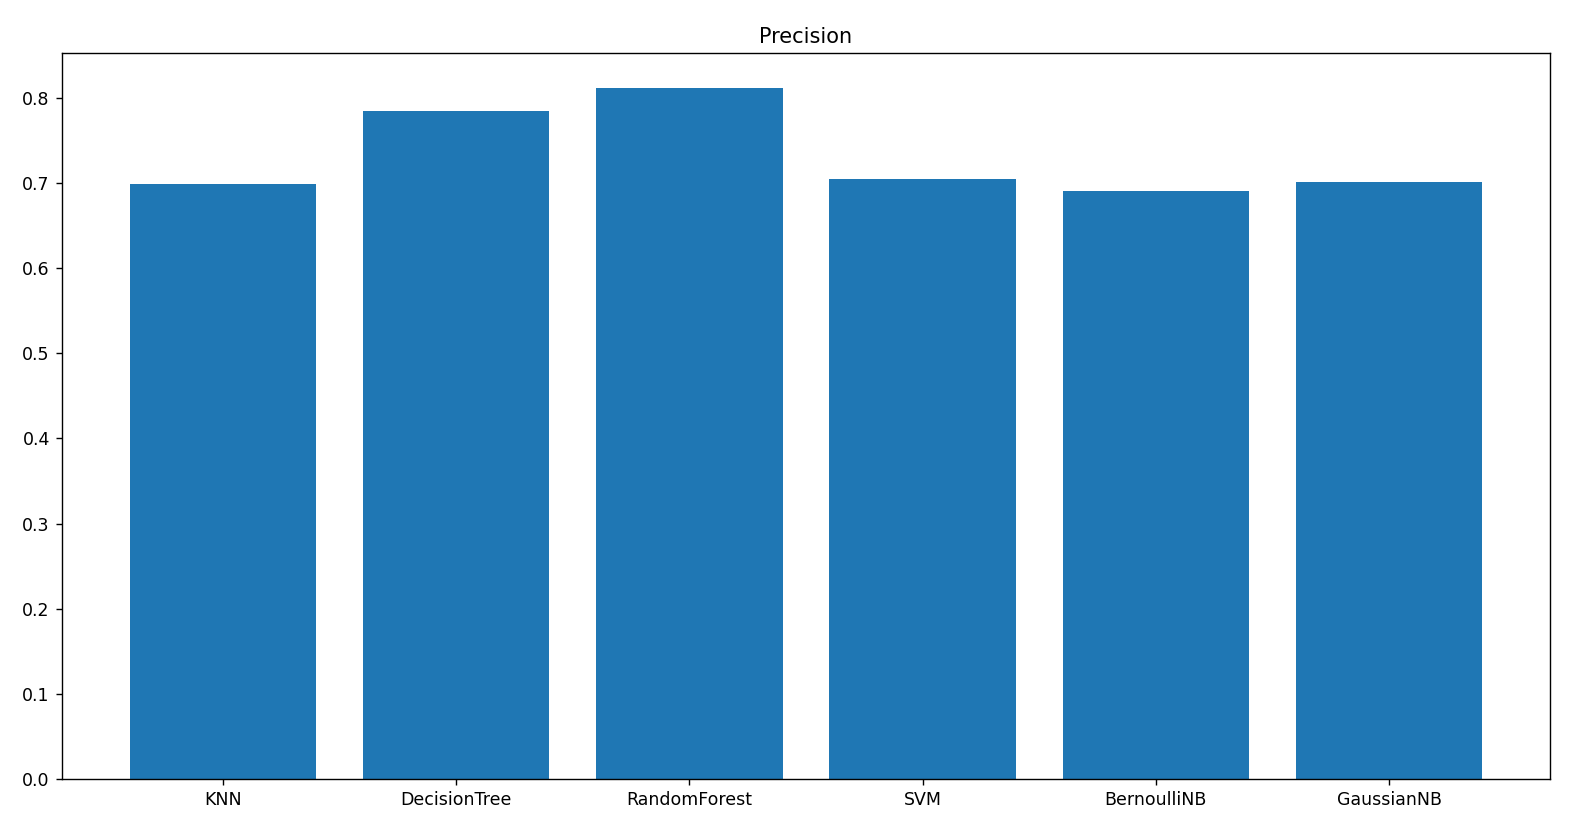
\includegraphics[width=0.9\textwidth]{Precision}
        \centering
        \caption{Grafico metrica precisione}
        \centering
\end{figure}

\begin{figure}[H]
        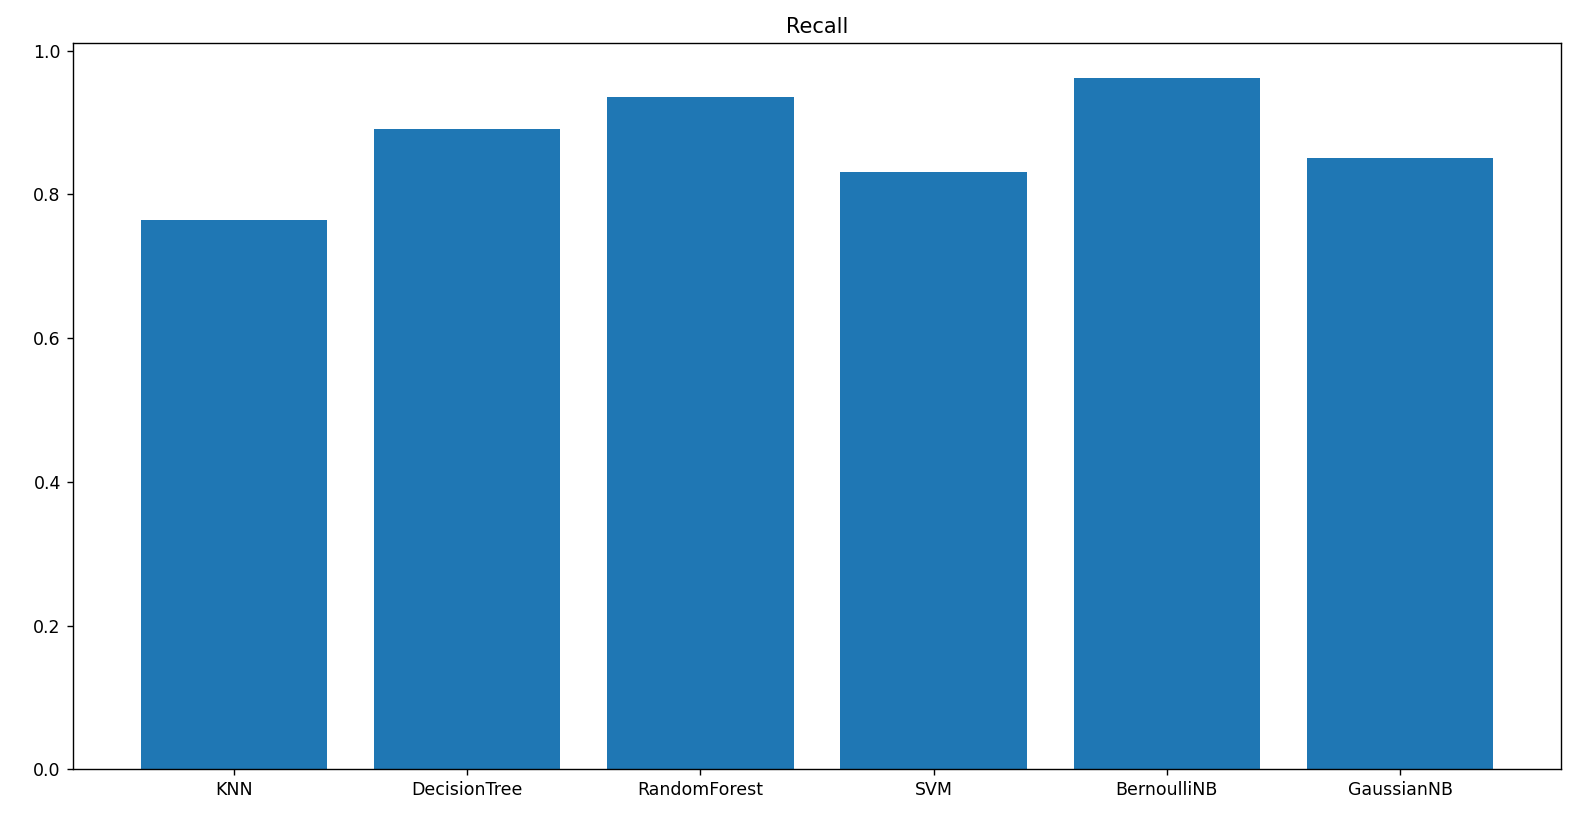
\includegraphics[width=0.9\textwidth]{Recall}
        \centering
        \caption{Grafico metrica richiamo}
        \centering
\end{figure}

\begin{figure}[H]
        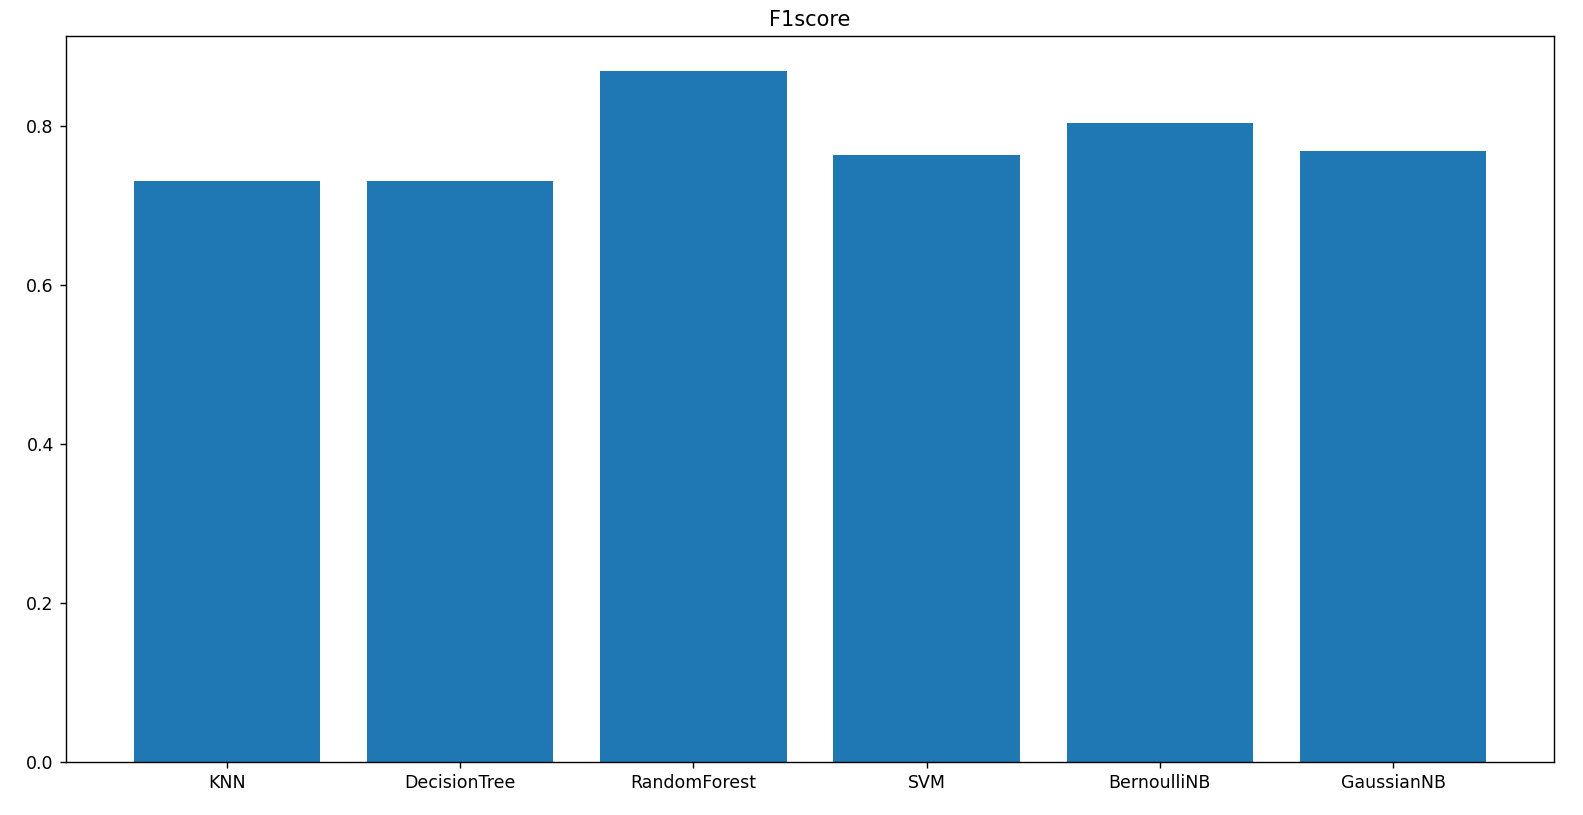
\includegraphics[width=0.9\textwidth]{F1score}
        \centering
        \caption{Grafico metrica F1-score}
        \centering
\end{figure}
%

\begin{figure}[H]
        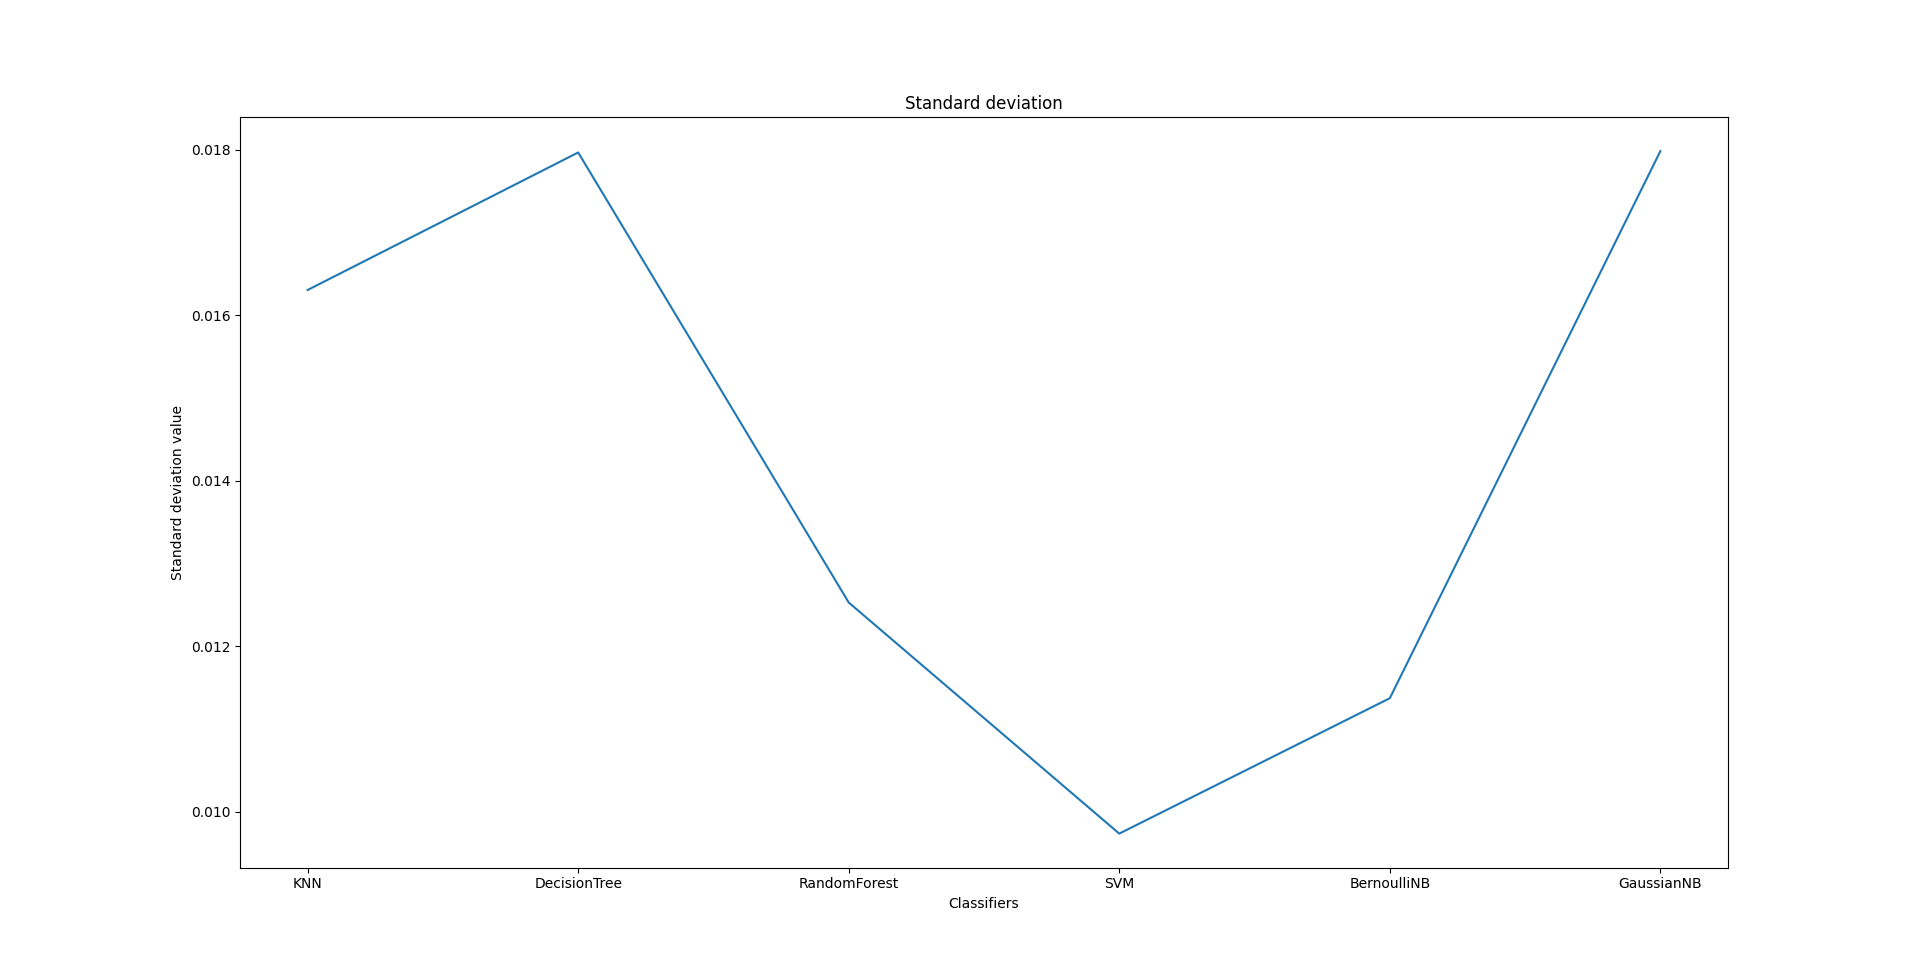
\includegraphics[width=0.9\textwidth]{dev2}
        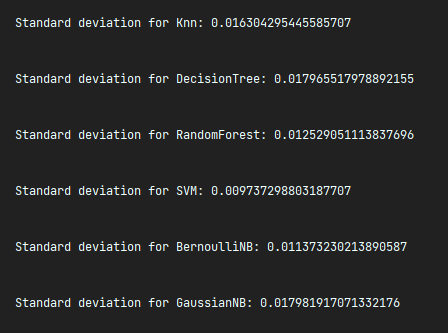
\includegraphics[width=0.5\textwidth]{dev1}
        \centering
        \caption{Deviazione standard dei classificatori}
        \centering
\end{figure}
%


\noindent
Basandoci su tali performance, in particolare su quella del \textbf{F1-score}, abbiamo riscontrato che il classificatore migliore risulta essere il Random Forest.

\subsection{Verifica dell'importanza delle features}
A seguito dell'analisi effettuata in precedenza, abbiamo generato un grafico che estrae le features più importanti derivanti proprio dal Random Forest:  

\begin{figure}[H]
        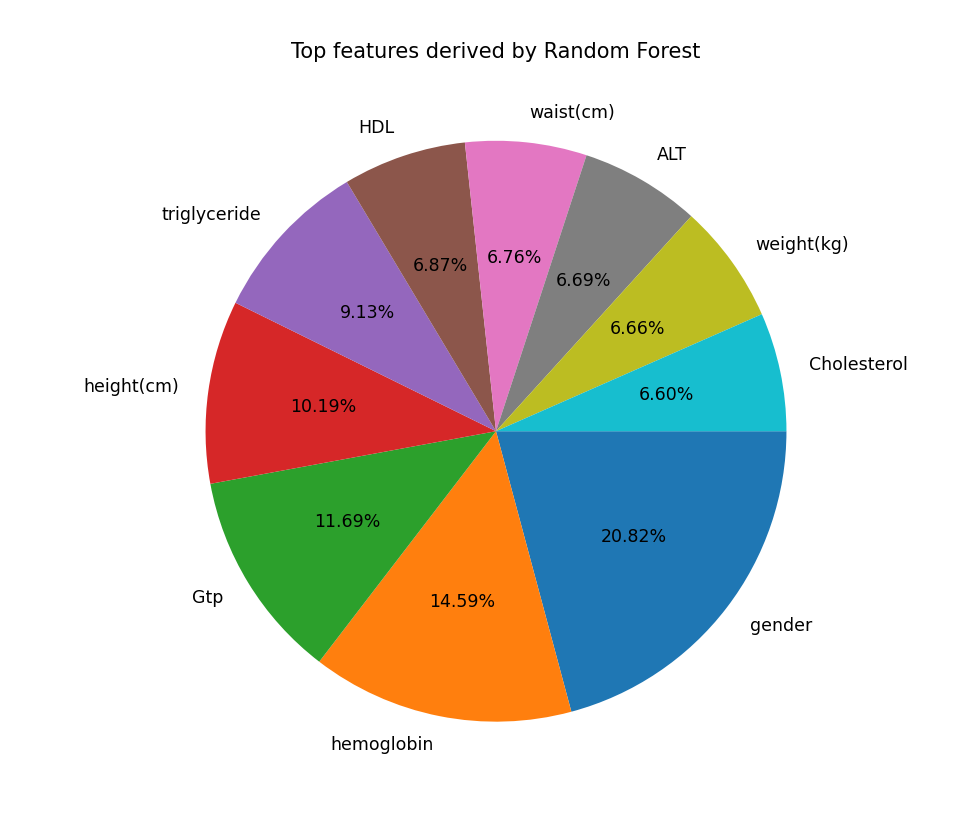
\includegraphics[width=0.9\textwidth]{Grafico3}
        \centering
        \caption{Risultati classificatore Random Forest}
        \centering
\end{figure}
%

\noindent
Possiamo notare che il genere, l'emoglobina e il gtp
sono le caratteristiche mediche predittive più importanti per la diagnostica di un soggetto potenzialmente fumatore o meno.

\subsection{Creazione della rete bayesiana}
Abbiamo scelto di implementare una rete bayesiana per poter effettuare delle interrogazione per
verificare le probabilità delle features, utilizzando come metodo di scoring il K2score.\\ 
Le tabelle CPD vengono generate con il dataset "smoking.csv" e andando ad usare il
MaximumLikeliHoodEstimator creiamo una rete bayesiana completa, con le probabilità apprese dal
dataset. In questo modo la predizione avverrà in base alle nostre features.\\
Dall'analisi delle rete è emerso che la feature \textit{oral} non ha nessun collegamento con gli altri nodi della rete. Mentre, le features \textit{Cholesterol} e \textit{LDL} hanno un collegamento tra loro ma sono scollegate dai restanti nodi della rete. Ragion per cui, si è optato per la loro eliminazione  e quindi, abbiamo effettuato una feature selection, in modo da poter ridurerre la complessità delle operazioni.
%

\begin{figure}[H]
        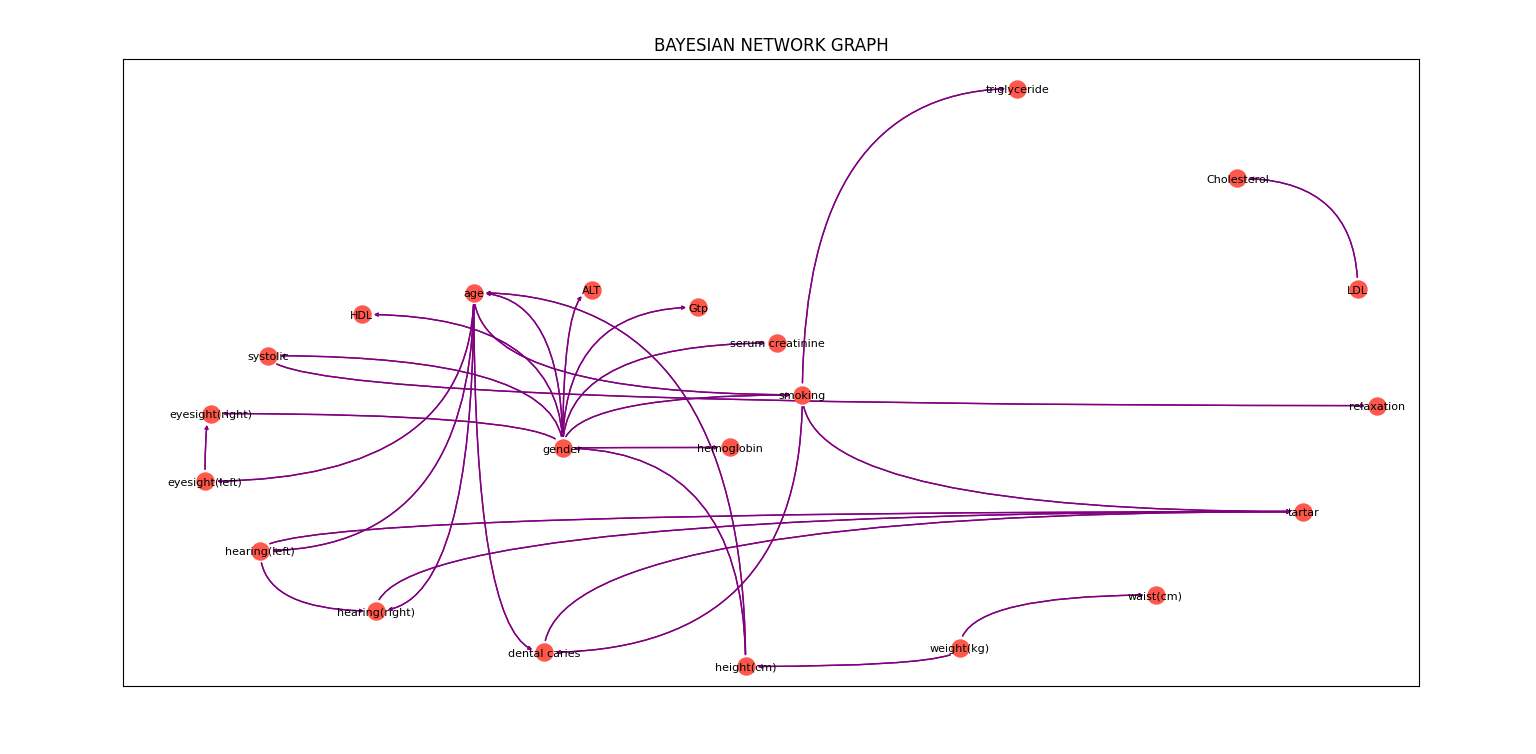
\includegraphics[width=16.5cm]{rete}
        \centering
        \caption{Grafo della rete bayesiana}
        \centering
\end{figure}
%


\subsubsection{Calcolo della probabilità}

Sfruttando la rete bayesiana precedentemente creata, calcoliamo le probabilità per le features \textit{gender} e \textit{smoking}.

\paragraph{Gender}
Dalle osservazioni precedenti è emerso che la feature \textit{gender} influenza diverse features, ragion per cui osserviamo con delle interrogazioni tali influenze.

\noindent
Data una variabile X, solo alcune variabili influenzano direttamente il suo valore.\\Le variabili che influenzano localmente sono dette \textit{Markov Blanket}.\\
Le Markov blanket di \textit{gender}, quindi, sono:

\begin{figure}[H]
        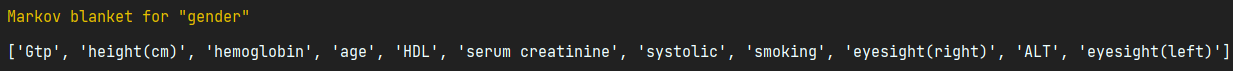
\includegraphics[width=0.9\textwidth]{MARKgen}
        \centering
        \caption{Markov blanket di \textit{gender}}
        \centering
\end{figure}

Tenendo in considerazione le Markov blanket di \textit{gender}, abbiamo effettuato interrogazioni sulla rete con un soggetto femminile ed uno maschile non fumatori. 

\begin{figure}[H]
        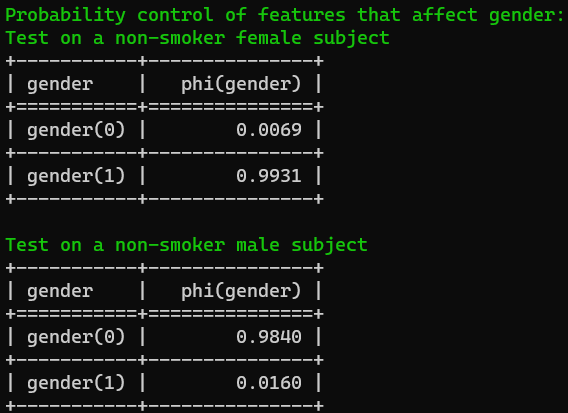
\includegraphics[width=10.6cm]{notSmokeGen}
        \centering
        \caption{Probabilità ottenute}
        \centering
\end{figure}

\noindent
N.B.\\Anche se i risultati delle probabilità, sono indicati con phi, tutte le probabilità calcolate sono probabilità condizionate.\\

Per ottenere tali dati, abbiamo effettuato le seguenti query:
\begin{enumerate}
    \item contenente i dati di un soggetto femminile;
    \item contenente i dati di un soggetto maschile.
\end{enumerate}
\begin{figure}[H]
        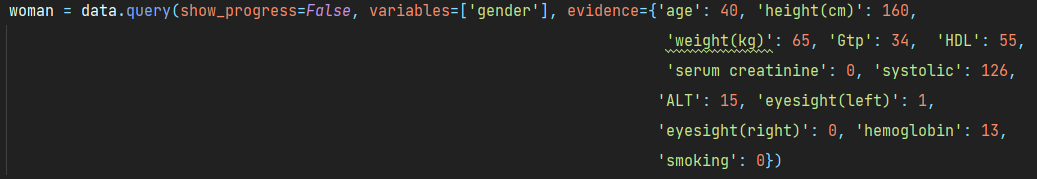
\includegraphics[width=0.9\textwidth]{queryWomanNoTSmoke}
        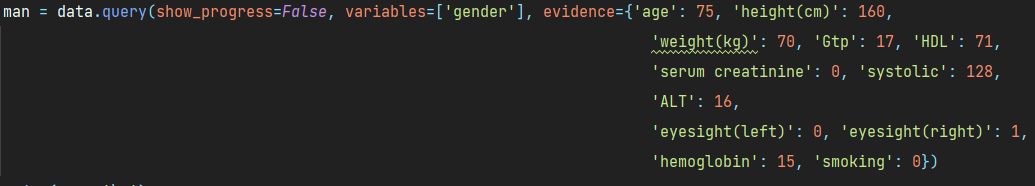
\includegraphics[width=0.9\textwidth]{queryManNoTSmoke}
        \centering
        \caption{Query effettuate}
        \centering
\end{figure}
%

Abbiamo effettuato le query sopra indicate, considerando i soggetti, questa volta, come fumatori.
Ottenendo come risultati:

\begin{figure}[H]
        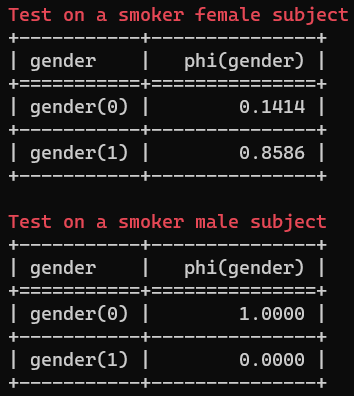
\includegraphics[width=10.6cm]{smokeGen}
        \centering
        \caption{Probabilità ottenute}
        \centering
\end{figure}


\paragraph{Smoking}

Le Markov Blanket di \textit{smoking}, invece, sono:

\begin{figure}[H]
        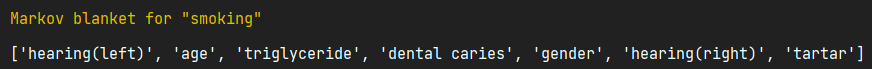
\includegraphics[width=0.9\textwidth]{MARK}
        \centering
        \caption{Markov blanket di \textit{smoking}}
        \centering
\end{figure}

%
Sfruttando la rete bayesiana, calcoliamo la probabilità per un soggetto presumibilmente non fumatore (0) ed uno fumatore (1) di esserlo o meno. Il soggetto di genere femminile preso in analisi ha età, altezza e peso standard, ovvero età: 20, altezza: 170, peso: 60.

\begin{figure}[H]
        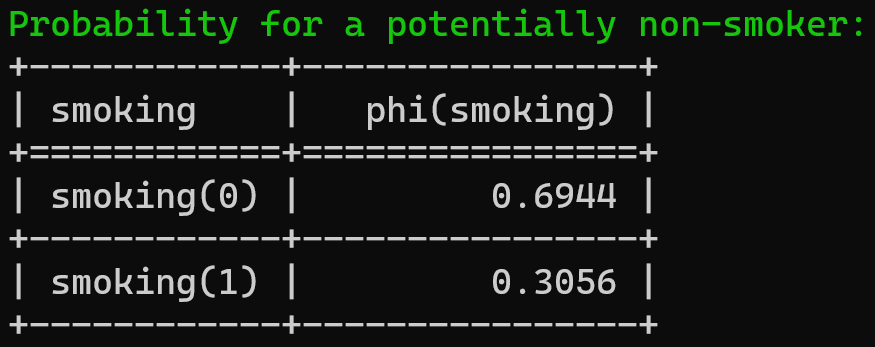
\includegraphics[width=10.6cm]{probNotSmoke}
        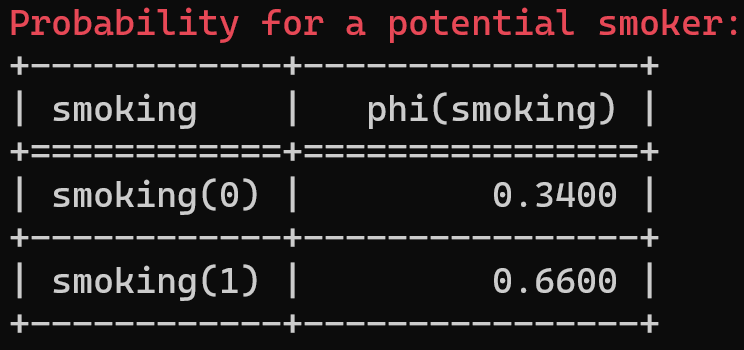
\includegraphics[width=10.6cm]{probSmoke}
        \centering
        \caption{Probabilità ottenute}
        \centering
\end{figure}

Per ottenere tali dati, abbiamo effettuato due query:
\begin{enumerate}
    \item contenente i dati di una persona non fumatrice;
    \item contenente i dati di una persona fumatrice.
\end{enumerate}
\begin{figure}[H]
        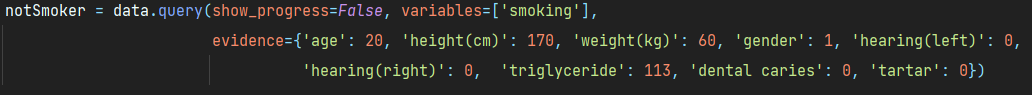
\includegraphics[width=0.9\textwidth]{queryNotSmoke}
        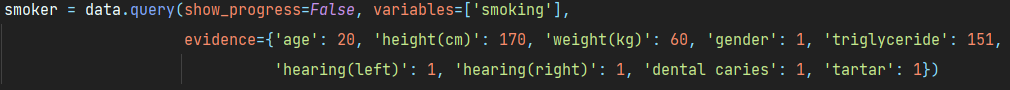
\includegraphics[width=0.9\textwidth]{querySmoke}
        \centering
        \caption{Query effettuate}
        \centering
\end{figure}
%

\noindent
Per verificare l'effettiva rilevanza delle features all'interno della rete bayesiana, abbiamo effettuato anche dei test sui soggetti presi in considerazione; riscontrando  che le features che influenzano maggiornamente risultano essere: \textit{triglyceride}, \textit{dental caries}, \textit{tartar}.   
%

\noindent
Ottenendo come probabilità:

\begin{figure}[H]
        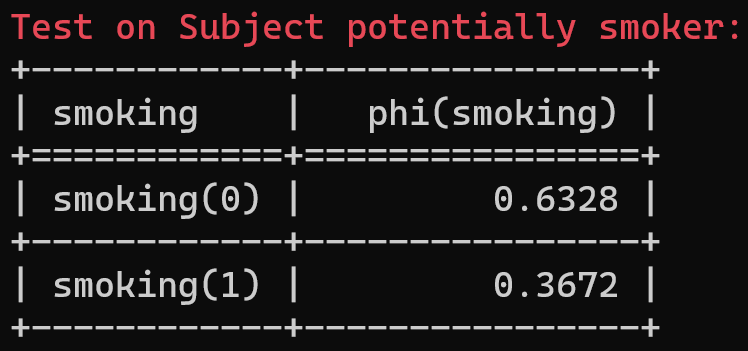
\includegraphics[width=10.6cm]{testSmoke}
        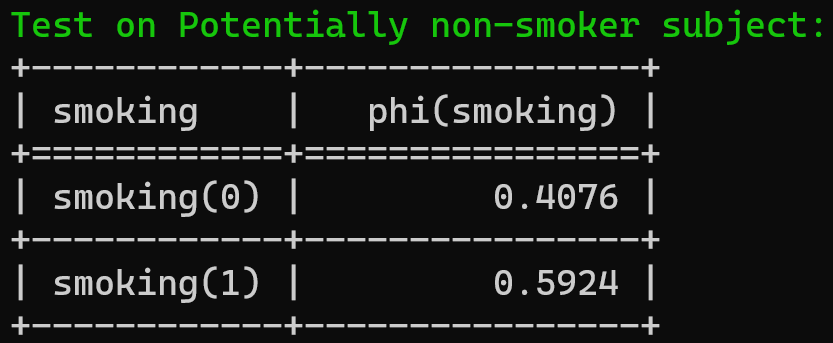
\includegraphics[width=10.6cm]{testNotSmoke}
        \centering
        \caption{Probabilità ottenute dai test}
        \centering
\end{figure}

\begin{figure}[H]
        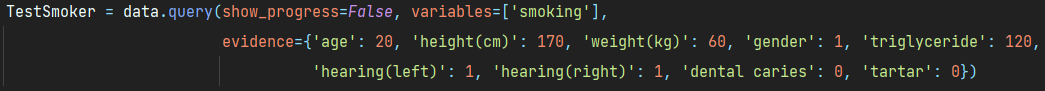
\includegraphics[width=0.9\textwidth]{queryTestSmok}
        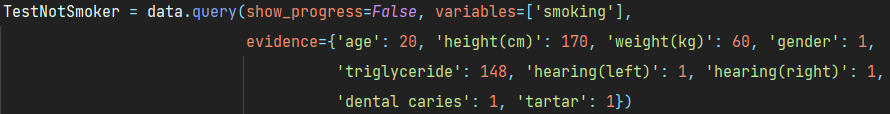
\includegraphics[width=0.9\textwidth]{queryTestNotSMok}
        \centering
        \caption{Query effettuate per i test}
        \centering
\end{figure}
%

\subsection{Interfaccia per l'interazione dell'utente con la knowledge base}

\begin{figure}[H]
        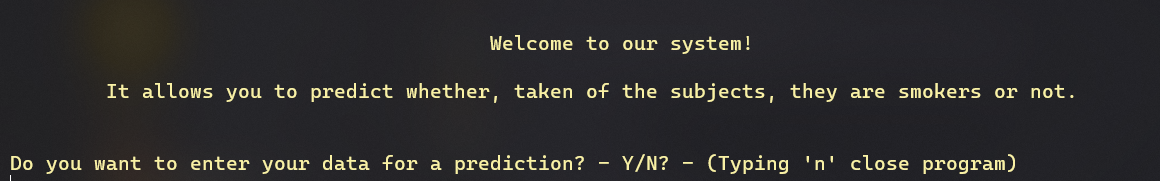
\includegraphics[width=0.9\textwidth]{welcome}
        \centering
        \caption{Interazione con la knowledge base}
        \centering
\end{figure}

L'utente può decidere di interagire con la knowledge base effettuando interrogazioni su quest’ultima. Per poterlo fare, bisogna inserire i dati relativi alla sua età, altezza, peso e genere obbligatoriamente (rispettando i valori ed i controlli segnalati, ove dovuti). Per i restanti valori, quali triglyceride, hearing(left), hearing(right), dental caries, tartar, l'utente se non è a conoscenza di uno di essi (o di tutti) può scegliere di non inserirli e quindi effettuare una interrogazione "parziale". Nell'eventualità che l'utente inserisca valori non validi o fuori range indicato, viene segnalato l'errore.

\begin{figure}[H]
        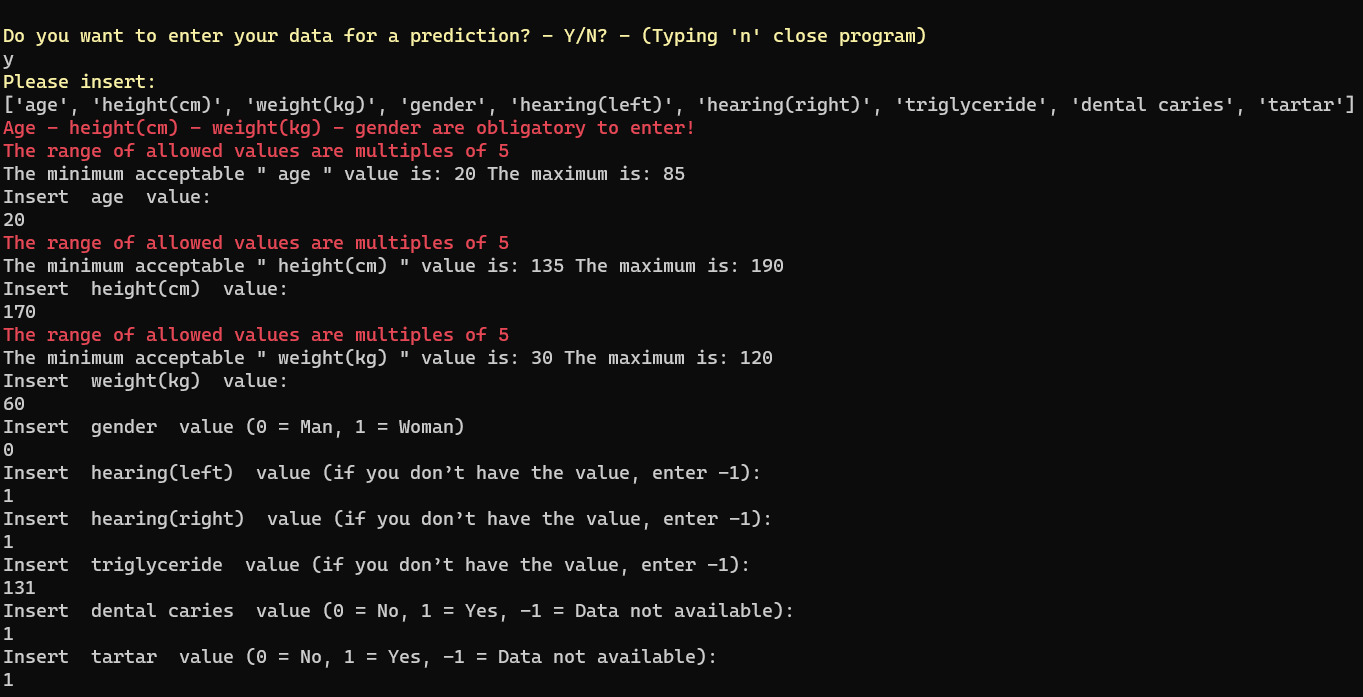
\includegraphics[width=0.9\textwidth]{interazione1}
        \centering
        \caption{Inserimento dei valori}
        \centering
\end{figure}
%

\noindent
Successivamente, viene visualizzata la probabilità risultante dai valori impostati dall'utente.

\begin{figure}[H]
        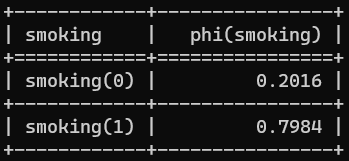
\includegraphics[width=10.6cm]{probility}
        \centering
        \caption{Probabilità a seguito dei valori inseriti dall'utente}
        \centering
\end{figure}
%

\noindent
Nel caso in cui la probabilità di essere un fumatore dovesse risultare superiore al 50\%, il sistema chiede all'utente se desidera riceve suggerimenti, ottenuti mediante una predizione, di valori ai quali ambire per poter risultare un non fumatore; tali valori sono ottenuti partendo dai valori di età, altezza, peso e genere.
Se il sistema dovesse trovare una combinazione valida, ovvero con probabilità inferiore al 50\%, viene visualizzata come segue:

\begin{figure}[H]
        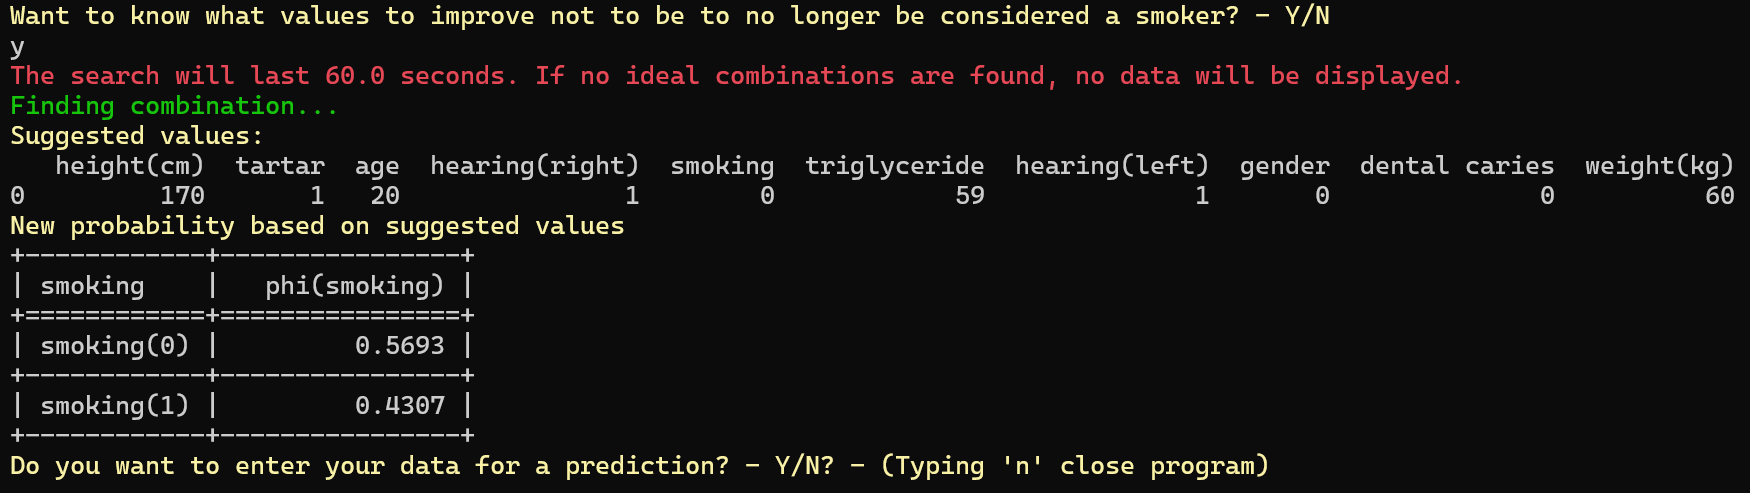
\includegraphics[width=0.9\textwidth]{search}
        \centering
        \caption{Valori suggeriti e nuova probabilità}
        \centering
\end{figure}

\newpage
\begin{thebibliography}{5}
        \bibitem{ref}
        Kompremos. (2020). Classificatore Naive Bayes. 
        \\\url{https://kompremos.com/it/classificatore-naive-bayes/} 
        
        \bibitem{ref}
        Elite Data Science. (2022). How to Handle Imbalanced Classes in Machine Learning. 
        \\\url{https://elitedatascience.com/imbalanced-classes} 
        
        \bibitem{ref}
        D. Poole, A. Mackworth: Artificial Intelligence: Foundations of Computational
        Agents. Cambridge University Press. 2nd Ed. [Ch.8]
        \\\url{http://artint.info/2e/html/ArtInt2e.Ch8.html} 
        
        \bibitem{ref}
        Documentazione libreria \textit{scikit-learn}.
        \\\url{https://scikit-learn.org/stable/user_guide.html} 
        
         \bibitem{ref}
        Documentazione libreria \textit{pgmpy}.
        \\\url{https://pgmpy.org/} 
        
        
        \end{thebibliography}

\end{document}